\documentclass[12pt]{report}

% Preambulo
\usepackage[frenchb]{babel}
\usepackage{float}
\usepackage[utf8]{inputenc}  
\usepackage{lmodern}
\usepackage[T1]{fontenc}  
\usepackage{graphicx}
\usepackage{indentfirst}
\usepackage{courier}
\usepackage{geometry}
\usepackage{glossaries}
\usepackage{eurosym}
\newcommand {\cod} [1] { \texttt {#1}} 
\newcommand {\p} [1] { \paragraph {#1}}
\usepackage{hyperref}
\hypersetup{
    colorlinks,
    citecolor=black,
    filecolor=black,
    linkcolor=black,
    urlcolor=black
}
\usepackage[backend=bibtex,urldate=comp,dateabbrev=false,sorting=none]{biblatex}
\bibliography{bibliographie.bib}

\title{Rapport de Stage 2A}
\author{Antônio Guilherme \textsc{Ferreira Viggiano}}
%\date{}
\makeindex
\geometry{paperwidth=210mm,paperheight=297mm,
  top=30mm,bottom=30mm,
  left=30mm,right=30mm}

\makeglossaries
\renewcommand*{\glspostdescription}{. Page:}

\begin{document}

\begin{titlepage}
\begin{center}
% Upper part of the page

\begin{figure}[ht]
  \begin{minipage}[b]{0.5\linewidth}
    \centering
    
\includegraphics[width=0.7\textwidth]{img/logo_ecm}
    \label{logo_ecm}
  \end{minipage}
  \hspace{0.5cm}
  \begin{minipage}[t]{0.5\linewidth}
    \vspace{-4cm}
    \begin{center}
    
\includegraphics[width=0.4\textwidth]{img/logo_asert}
    \end{center}
    \label{logo_asert}
  \end{minipage}
\end{figure}

%\textsc{\LARGE Intelligence Artificielle et Prolog}\\[1.5cm]


% Title
\vspace{2cm}
\hrule  ~\\[0.4cm]
{ \huge \bfseries Stage assistant ingénieur en développement logiciel}\\[0.4cm]

\hrule  ~\\[0.5cm]

\textsc{\LARGE Rapport de stage deuxième année}\\[1.5cm]


\end{center}


\vfill


\large\emph{Elève :} \hfill Antônio Guilherme \textsc{Ferreira Viggiano} ~\\

\large\emph{Tuteur pédagogique :} \hfill M. Pascal \textsc{Préa}

\large\emph{Tuteur de stage :} \hfill M. Clemenceau Roberto \textsc{Da Silva}

\vfill

\begin{center}
  \large Stage realisé du 3 Juin au 26 Juillet \\
  (8 semaines)
\end{center}






\end{titlepage}


\pagebreak
%!TEX root = index.tex

%Entradas do glossário
\newglossaryentry{eclipse}
{
  name=Eclipse,
  description={-- Environnement de développement intégré multi-langage comprenant un espace de travail de base et une extensible système plug-in de personnalisation de l'environnement. Écrit en Java, il peut être utilisé pour développer des applications en Java et d'autres langages de programmation}
}

\newglossaryentry{jee}
{
  name=Java EE,
  description={-- La plate-forme informatique Java d'Oracle destinée aux entreprises. La plate-forme fournit une API et un environnement d'exécution pour l'élaboration et la mise en œuvre du logiciel d'entreprise, y compris les services de réseau et web, et d'autres applications de réseau à grande échelle, multi-niveaux, évolutive, fiable et sécurisée.}
}

\newglossaryentry{SGBD}
{
  name=SGBD,
  description={-- Système de Gestion de Base de Données, est un logiciel système destiné à stocker et à partager des informations dans une base de données, en garantissant la qualité, la pérennité et la confidentialité des informations, tout en cachant la complexité des opérations.}
}

\newglossaryentry{plug-in-hybrid}
{
  name=plug-in hybrid,
  description={-- Hybrid vehicle that uses batteries which can be fully recharged by connecting a plug to an external power source, either at home or at a power station. This is used to reduce costs related to battery replacement and to enable all-electric operation, reducing greenhouse gas emissions},
  plural=plug-in hybrids
}

\newglossaryentry{Better-Place}
{
  name=Better Place,
  description={-- An international company that developed and sold battery-switching battery for electric cars. The corporation did not succeed mainly because of non-standardization of battery models, and has declared bankruptcy in Israel and has initiated the proceedings in Denmark},
}


\newglossaryentry{frunk}
{
  name=frunk,
  description={-- The front trunk. Electric vehicles are usually able to have both rear and front trunks because the batteries are located in the floor, and the motor between the drive wheels},
}

\newglossaryentry{hybrid}
{
	name=hybrid car,
	description={-- Vehicle that uses more than one power source to move the wheels. Most commonly, it refers to hybrid electric vehicles, which combine internal combustion engines and electric motors}
}

\newglossaryentry{li-ion}
{
	name=lithium-ion battery,
	description={-- A rechargeable battery used to power electric vehicles. Li-ion batteries have high energy density and slow self-discharge when not in use, and are known for being more expensive than older nickel metal batteries},
	plural=lithium-ion batteries
}

\newglossaryentry{range-extender}
{
	name=range extender,
	description={-- A system used in hybrid cars where the internal combustion engine is used solely to charge up the battery, and not to power the wheels. This system is used as an emergency tool, when battery is running out of charge},
	plural=range extenders
}

\newglossaryentry{range-anxiety}
{
	name=range anxiety,
	description={-- An expression used to designate a driver's worry that his vehicle won't reach its destination on the current charge, especially because of battery charge restrictions and limited electric power stations on the way}
}

\newglossaryentry{zero-emission}
{
	name=zero-emission vehicle,
	description={-- A vehicle that has zero gas emissions at the tailpipe. Emissions from the manufacturing process are whatsoever ignored in this definition},
	plural=zero tailpipe emissions
}

\newglossaryentry{gas-emission}
{
	name=greenhouse gas,
	description={-- Gas substance (such as water vapor or carbon dioxide) that absorb part of the infrared radiation emitted by the surface of Earth. This process decreases heat loss, keeping the planet warm. Human activities such as industrial or tailpipe emissions increase greenhouse gases concentration on air, changing Earth's average temperature},
	plural=greenhouse gas emissions
}

\newglossaryentry{fuel-cell}
{
	name=fuel cell,
	description={-- Device capable of converting chemical energy into electricity. An electrolyte initiates a chemical reaction that generates electric power when fuel and oxidants, such as hydrogen and oxygen, flow into it. While no greenhouse gases are produced in the process, hydrogen production and distribution may have a significant environmental impact}
}

\newglossaryentry{government-incentives}
{
	name=government incentives,
	description={-- Subsidies or government policies beneficial for electric cars, which vary with federal government and vehicle model. Most incentives are tax credits and personal income tax deduction for costumers},
	plural=government policy
}

\newglossaryentry{bev}
{
	name=battery electric vehicle,
	description={-- Also referred to as all-electric vehicle, it is a vehicle that is use a battery as the only mean to store electricity needed to power the motor},
	plural=battery electric vehicles
}



\pagebreak
\section*{Remerciements}

Je voudrais remercier à tous ceux qui ont contribué pour le bon déroulement de ce stage, en particulier à :

\vspace{1em}

\begin{description}
\item[Mme Mirta JUAREZ et Mme Cécile LOUBET --] pour les réponses rapides à toute question concernant le stage à l'international.
\item[M. Marco Aurélio RABELO --] président-directeur général de Asert, pour être si proche des employés.
\item[M. Clemenceau Roberto DA SILVA --] directeur de technologie de l'entreprise, qui m'a bien accueilli par email et personnellement au sein de l'entreprise.
\item[M. Thiago RODRIGUES PEREIRA --] architect logiciel, pour m'avoir formé dans le framework de l'entreprise et m'avoir introduit aux bonnes pratiques en génie logiciel.
\end{description}


\pagebreak
\chapter*{Résumé}

Ce rapport décrit un stage technique d'assistant ingénieur d'une durée de deux mois au sein de Asert Serviços e Tecnologia da Informação (Asert Services et Technologies de l'Information). Cette entreprise de petite taille située à Goiânia, la capitale de l'état brésilien Goiás, offre des solutions de développement de technologies et externalisation de services informatiques, et est spécialisée en services d'aide médicale. 

Le poste qui m'a été affecté a été celui de développeur logiciel dans le Centre de Développement de Services de la société, où j'ai travaille essentiellement avec les langages de programmation Java et Flex. Ces technologies ont été utilisées pour l'élaboration d'un portail web Flash de gestion de personnes adhérentes à la société d'assurance mutuelle Celgmed, une mutuelle de santé destinée aux employés de CELG, la Compagnie Énergétique de Goiás, similaire à Électricité de France S.A.

Le mode de fonctionnement de l'entreprise, sa taille, son marché et ses produits seront également présentés en détail, aussi bien que sa politique concernant l'hygiène, la sécurité au travail et le climat social. Les remarques personnelles de l'élève et l'apport de cette expérience seront discutés dans la conclusion de ce rapport.


\chapter*{Abstract}

\begin{center}
\bfseries retraduzir
\end{center}

This report describes a two-month technical internship as an engineer assistant at Asert Serviços e Tecnologia da Informação, a small software development company that provides outsourcing and IT services, specialized in medical services. This internship took place at Goiânia, the capital of the Brazilian state of Goiás. The functions I executed were in the Services Development Center, where I worked as a software developer mostly in Java and Flex, two of the technologies which will be discribed later. The mode of operation of the company, its size, its market and its products will be presented in
detail, as well as its policy concerning hygiene, safety and social climate. Personal remarks of the student and the contribution of this experiment will be discussed in the conclusion of this report.


\pagebreak
\section*{Mots clefs}

\begin{itemize}
\begin{itemize}
\item Stage assistant ingénieur
\item Asert Serviços e Tecnologia da Informação
\item École Centrale Marseille
\item Externalisation de services
\item Systèmes de gestion intégrés
\item Audit en services d'aide médicale
\item Portail web
\item Java
\item Flex
\item Flash
\end{itemize}
\end{itemize}


\pagebreak
%!TEX root = index.tex

%Entradas do glossário
\newglossaryentry{EV}
{
  name=EV,
  description={-- Electric Vehicle. A vehicle that uses one or more electric motors or traction motors for propulsion. Electric vehicles include cars, trains, trucks, planes, boats, motorcycles, among others. The term is frequently interchanged with electric cars, designating battery-only cars or hybrid electric cars},
  plural=EVs
}

\newglossaryentry{energy-mix}
{
  name=energy mix,
  description={-- The many energy sources of a region, either renewable or non-renewable. Theses may include coal, biomass, diesel, wave power, wind energy, etc}
}

\newglossaryentry{well-to-wheel}
{
  name=well to wheel,
  description={-- The life-cycle analysis used to evaluate environmental impacts associated with all stages of a vehicle's life. This would include in particular gas emissions in the process of powering up batteries and transporting them}
}

\newglossaryentry{plug-in-hybrid}
{
  name=plug-in hybrid,
  description={-- Hybrid vehicle that uses batteries which can be fully recharged by connecting a plug to an external power source, either at home or at a power station. This is used to reduce costs related to battery replacement and to enable all-electric operation, reducing greenhouse gas emissions},
  plural=plug-in hybrids
}

\newglossaryentry{Better-Place}
{
  name=Better Place,
  description={-- An international company that developed and sold battery-switching battery for electric cars. The corporation did not succeed mainly because of non-standardization of battery models, and has declared bankruptcy in Israel and has initiated the proceedings in Denmark},
}


\newglossaryentry{frunk}
{
  name=frunk,
  description={-- The front trunk. Electric vehicles are usually able to have both rear and front trunks because the batteries are located in the floor, and the motor between the drive wheels},
}

\newglossaryentry{hybrid}
{
	name=hybrid car,
	description={-- Vehicle that uses more than one power source to move the wheels. Most commonly, it refers to hybrid electric vehicles, which combine internal combustion engines and electric motors}
}

\newglossaryentry{li-ion}
{
	name=lithium-ion battery,
	description={-- A rechargeable battery used to power electric vehicles. Li-ion batteries have high energy density and slow self-discharge when not in use, and are known for being more expensive than older nickel metal batteries},
	plural=lithium-ion batteries
}

\newglossaryentry{range-extender}
{
	name=range extender,
	description={-- A system used in hybrid cars where the internal combustion engine is used solely to charge up the battery, and not to power the wheels. This system is used as an emergency tool, when battery is running out of charge},
	plural=range extenders
}

\newglossaryentry{range-anxiety}
{
	name=range anxiety,
	description={-- An expression used to designate a driver's worry that his vehicle won't reach its destination on the current charge, especially because of battery charge restrictions and limited electric power stations on the way}
}

\newglossaryentry{zero-emission}
{
	name=zero-emission vehicle,
	description={-- A vehicle that has zero gas emissions at the tailpipe. Emissions from the manufacturing process are whatsoever ignored in this definition},
	plural=zero tailpipe emissions
}

\newglossaryentry{gas-emission}
{
	name=greenhouse gas,
	description={-- Gas substance (such as water vapor or carbon dioxide) that absorb part of the infrared radiation emitted by the surface of Earth. This process decreases heat loss, keeping the planet warm. Human activities such as industrial or tailpipe emissions increase greenhouse gases concentration on air, changing Earth's average temperature},
	plural=greenhouse gas emissions
}

\newglossaryentry{fuel-cell}
{
	name=fuel cell,
	description={-- Device capable of converting chemical energy into electricity. An electrolyte initiates a chemical reaction that generates electric power when fuel and oxidants, such as hydrogen and oxygen, flow into it. While no greenhouse gases are produced in the process, hydrogen production and distribution may have a significant environmental impact}
}

\newglossaryentry{government-incentives}
{
	name=government incentives,
	description={-- Subsidies or government policies beneficial for electric cars, which vary with federal government and vehicle model. Most incentives are tax credits and personal income tax deduction for costumers},
	plural=government policy
}

\newglossaryentry{bev}
{
	name=battery electric vehicle,
	description={-- Also referred to as all-electric vehicle, it is a vehicle that is use a battery as the only mean to store electricity needed to power the motor},
	plural=battery electric vehicles
}



\pagebreak
\tableofcontents

\pagebreak
\chapter{Introduction}

L'École Centrale Marseille propose dans son cursus aux élèves de découvrirent le monde économique et ses contraintes et de bien appréhender la complexité du métier d'ingénieur, au travers d'un stage en entreprise d'une durée de 8 semaines au minimum. Celle-ci est une opportunité complémentaire au stage ouvrier de la première année extrêmement enrichissante dans plusieurs aspects. 

Ce rapport présente les expériences dans l'établissement Asert Serviços e Tecnologia da Informação, une petite société informatique qui propose des solutions de systèmes de gestion intégrés à d'autres entreprises, principalement à celles d'aide médicale.

Le déroulement de ce stage a été du 3 juin 2013 au 26 juillet 2013, avec une durée totale de huit semaines, où j'ai occupé le poste de développeur logiciel dans le Centre de Développement de Systèmes à Asert. 

Ce document a pour objectif montrer de façon détaillée les expériences vécues lors du stage, et pour cella il est divisé en trois parties :  la présentation de l'entreprise, la description du poste occupée, avec une mise en évidence du processus de développement logiciel, et la conclusion contenant les remarques personnelles de l'élève en ce qui concerne cette expérience.


\pagebreak
\chapter{Présentation de l’entreprise}
\section{Historique}

Basée dans la capitale de Goiás, Asert a été fondée en 2002 par deux employés de Evoluti Tecnologia e Serviços (Evoluti Technologie et Services) avec l'idée de fournir des systèmes de gestion au secteur de la santé, un domaine qui ne possédait pas les compétences techniques nécessaires à l'intégration de tous ses services. Tout de même, Asert n'a éte qu'une branche rattachée à Evoluti jusqu'en 2008, lorsque l'entreprise a réussi à avoir suffisamment de projets indépendants.

De 2008 à 2010, la société a travaillé fondamentalement avec des systèmes pour des mutuelles de santé. Récemment, suivant les tendances du marché, l'organisation a élargi son champ d'application jusqu'à l'externalisation de tout type de service spécialisé.

\section{Implantation et Taille}

Asert est une micro-entreprise localisée dans la région commerciale de Goiânia, dans un bureau d'approximativement 110 m$^2$, actuellement avec un effectif de 12 employés. En 2010, grâce à un projet en partenariat avec l'état de Goiás, l'entreprise comptait 200 personnes, y compris des médecins, des auditeurs et consultants, des professionnels de TI, etc. Cependant, à la fin de l'engagement, Asert a dû mettre à terme les contrats de travail à durée déterminée et rester avec son équipe principale.

\section{Type de structure}

L'entreprise se partage en deux secteurs, le Centre de Développement de Systèmes, où quatre développeurs sont gérés par un chef d'équipe, et le Centre Commercial-Financier, où des commerciaux, compteurs et administrateurs sont dirigés par le directeur financier.

L'équipe commerciale se charge de trouver de nouveaux clients et de faire une analyse préalable de la situation de l'entreprise. Le chef de projets du centre de développement fait ensuite l'analyse technique du système de gestion souhaité, en prenant note de toutes les particularités spécifiques aux règles métier (ou ``business rules'' en anglais) règle-métier de l'application. Une fois le besoin du client complètement identifié, l'équipe de développement décide la structure ``physique'' du système -- quelle base de données relationnelle utiliser, quelle langage de programmation ou technologie la plus adaptée au problème, etc. -- et passe à l'étape de codage.

L'équipe financière travaille en parallèle de toutes ces étapes, en analysant les coûts de travail et d'équipements.

\section{Gamme de produits}

Même si Asert est spécialisée en services de santé, le groupe travaille  sur deux grandes gamme de projets, ceux de technologies et de l'information et ceux de systèmes intégrés. 

\subsection{Technologies de l'information}

Dans l'axe des sciences de l'information et de la communication, l'entreprise propose des services de audit et conseil, de développement de systèmes, d'informatique décisionnelle (en anglais \textit{Business Intelligence}) et de gestion.

\subsubsection{Audit et conseil}

Le rôle du conseil en technologies de l'information est de fournir au client un bilan de la situation actuelle de l'entreprise, d'identifier les problèmes liés à la politique, à la structure, aux procédures et aux méthodes, afin de recommander et d'aider à mettre en \oe{}uvre les mesures appropriées aux étapes d'innovation et de croissance de l'entreprise. Après ce diagnostic fondé sur le besoin du client et les résultats attendus, Asert s'occupe du développement de solutions spécialisées et de projets techniques, avec des professionnels qualifiés au travail. Le service de \textit{consulting} comprend :

\begin{itemize}
\item Mise à niveau et modernisation de la technologie de la société;
\item Évaluation, sélection et embauche de services et logiciels tiers;
\item Préparation de projets de logiciels;
\item Gestion de projets.
\end{itemize}

\subsubsection{Développement de systèmes}

Ce n'est pas toujours que les systèmes de gestion disponibles sur le marché répondent aux demandes des organisations. C'est en vue de cela que Asert propose des systèmes sur mesure, en produisant des outils personnalisés en fonction des besoins des clients, de manière à assurer une plus grande productivité et amélioration de la gestion internet des entreprises.

Asert utilise les plus modernes méthodologies de développement logiciel, utilisant des méthodes de contrôle de version et de testes unitaires afin d'avoir un rendu selon les exigences et les besoins des clients.

\subsubsection{Informatique décisionnelle -- \textit{Business Intelligence}}

Les systèmes d'information sont responsables par la manipulation d'une quantité de données très importante au sein des entreprises. L'informatique décisionnelle, aussi connue par la traduction anglaise ``intelligence d'affaires'', est le processus de collecte, d'organisation, d'analyse, de partage et de suivi de ces données, afin d'extraire des informations et des indicateurs pour soutenir la gestion de l'établissement. Les services B.I. de Asert incluent :

\begin{itemize}
\item Analyse et conception d'environnements de gestion de l'information;
\item Analyse de la qualité des données;
\item Gestion des données;
\item Rendu de rapports dynamiques destinés aux gestionnaires de l'entreprise.
\end{itemize}

\subsubsection{Gestion des T.I.}

L'équipe de Asert est axée sur la satisfaction du client, prête à résoudre les difficultés dans l'accès ou l'utilisation des technologies de l'information. Elle fournit également aux utilisateurs un centre d'assistance pour résoudre à tout problème technique lié à ses services, afin de rétablir le fonctionnement normal des activités dès que possible, minimisant ainsi les impacts commerciaux causés par des pannes informatiques.

La gestion des technologies de l'information apporte plusieurs avantages aux organisations, comme la construction d'un lien entre les T.I. et la gestion d'entreprise, la réduction des coûts, l'acheminement des appels aux équipes spécialisées, le soutien aux utilisateurs finaux  et l'amélioration de la qualité des services.

\subsection{Systèmes Intégrés}

Les systèmes intégrés de l'entreprise se partagent en deux secteurs : la médecine, celle-ci divisé en Asert Santé et Asert Méd, et l'industrie, avec Asert Cycle.

\subsubsection{Asert Santé}

Asert Santé est le type de système informatisé pour la gestion des sociétés d'assistance médicale. Développé avec les technologies les plus modernes, le système se traduit par un portail web comme interface d'administration d'utilisateurs et d'adhérents, et de bases de données relationnelles qui manipulent toutes les informations. Ces systèmes sont en conformité avec les spécifications de l'Agence Nationale de Santé brésilienne.

Ces caractéristiques techniques, alliées à une interface conviviale et intuitive, rend le système facile à utiliser, sans demander beaucoup de ressources matérielles. Techniquement, le système est divisé en modules indépendants, qui sont intégrés selon la réalité et l'organisation de l'entreprise de santé. Ce type de développement ``en couches'' sera détaillé par la suite. 

Les particularités de Asert Santé sont :

\begin{itemize}
\item Modules intégrés;
\item En accord avec les normes de l'Agence Nationale de Santé brésilienne;
\item Rapidité, efficacité et fiabilité dans les tâches effectuées;
\item Vérification électronique;
\item Normalisation des tables de facturation et des rapports de gestion;
\item Facturation électronique.
\end{itemize}


\begin{figure}[hb]
\begin{center}
    
\includegraphics[scale=1.0]{img/asert-saude}
	\label{asert-saude}
\end{center}
\end{figure}

\subsubsection{Asert Méd}

Asert Méd est un outil idéal pour la gestion des cliniques, des hôpitaux, des laboratoires et des bureaux de médecin. Ce système vise à faciliter le service clients, la facturation et la présentation des comptes, adapté aux besoins du client.

Caractéristiques et avantages:

\begin{itemize}
\item Modules intégrés;
\item En accord avec les normes de l'Agence Nationale de Santé brésilienne;
\item Enregistrement unique des patients;
\item Assistance aux patients affiliés ou adhérents à une mutuelle de santé;
\item Émission de demandes de visites médicales dans les modèles des normatifs;
\item Contrôle des rapports médicaux personnalisés et de factures de soins médicaux et hospitaliers;
\item Contrôle des stocks multiple (entrepôt, pharmacie, soins infirmiers, etc.);
\item Gestion financière;
\item Graphiques et rapports de gestion;
\item Dossier médical électronique d'un patient.
\end{itemize}

\begin{figure}[hb]
\begin{center}
    
\includegraphics[scale=1.0]{img/asert-med}
	\label{asert-med}
\end{center}
\end{figure}

\subsubsection{Asert Cycle}

Asert Cycle est un système développé avec les dernières technologies sur le marché pour la gestion d'industries, permettant de façon innovante le contrôle, le suivi et l'intégration des politiques de management, de production, de commerce et fiscales des entreprises. Ce système se caractérise par :

\begin{itemize}
\item Gestion de stock;
\item Suivi du produit dans toutes les étapes de fabrication;
\item Expédition et vente des produits;
\item Émission de la facture;
\item Gestion de la production.
\end{itemize}

\section{Marché}
\subsection{Le marché des technologies de l'information et communication au Brésil}

Le marché des TIC au Brésil est composé de 99 \% de petites et moyennes entreprises et est actuellement en croissance, même si cela n'est pas un secteur traditionnel de l'économie du pays. En 2010, les technologies de l'information et communication ont été responsables par 102,6 milliard de dollars, environ 3\% \cite{pib-brasil} du produit intérieur brut \cite{uol-mercado-tic} de l'année. 



%8. mercado
%	mercado de TI no brasil: 99\% das empresas brasileiras sao MPE, micro e pequenas empresas, com poucos funcionarios e, dessas, 90\% fecham em %5 anos. Dificuldades tributarias, burocraticas, de implantacao no mercado, etc.


\subsection{La position de Asert dans le marché}

Dans les années 1990 et 2000, le boom des des progiciels de gestion intégré (ou en anglais ERP,  ``Enterprise Resource Planning'') a encouragé la création de plusieurs entreprises de de logiciels en tant que service (de l'anglais ``Software as a Service'', SaaS) dans l'état de Goiás, tels que Canion Software, Interagi Tecnologia, et Apta. Cependant, ce phénomène de haute concurrence a fait tomber les prix des ERPs et a empêché la croissance des petites et moyennes entreprises de technologie.

Ce que l'on constate aujourd'hui est le retour aux systèmes personnalisées. Les clients sont plus exigeantes dans les systèmes adaptés et ne veulent plus de logiciels génériques, souvent critiqués d'être de difficile adaptation et de ne pas représenter l'identité de l'entreprise. Avec ce changement de valeurs du marché, Asert a gagné de nouveaux clients et a assuré sa position en tant qu'entreprise de développement de solutions individualisées.

%..	buscando novos clientes (antigos usuarios de ERP que tao procurando algo mais personalizado). Esse systeme expert da friboi nao existe em lugar nenhum do mundo (por ser bastante especifico) e � um novo produto: � uma das maiores apostas da Asert no momento.

%pouco tempo atr�s: boom dos ERPs, fez diminuir bastante o preco de todos sitemas de gestao. todavia, dificil/cara adaptacao selon les caracteristiques du client. chaque entreprise tem a sua cara
%hoje: retorno devagar a sistemas personalizados

%BPO e BPM. http://processplatsen.ibissoft.se/?q=en/node/40

%ha apenas uma concorrencia direta, do Paran�, que tamb�m � uma empresa especializada em softwares de gestao de planos de saude, mas eles nao tem uma grande implantacao em Goi�s.

Au cours du temps, les projets de Asert ont évolué non pas seulement en taille mais aussi en type. Lorsque l'entreprise était rattaché au groupe Evoluti. Le premier projet de Asert a été la mise en ouvre d'un système de gestion pour l'association d'assistance médicale ``Ipasgo'' (Institut de l'assistance publique de l'Etat de Goias). Ensuite, le système s'est adapté à la ville de Palmas, capitale de l'état de Tocantins. Aujourd'hui ces deux projets sont en phase d'assistance -- l'étape finale de toutes les solutions d'externalisation de l'entreprise.

Actuellement, l'entreprise subit des transformations structurelles afin de pouvoir agir comme un moteur d'innovation de l'état. En partenariat avec l'institution gouvernementale FAPEC et avec l'institution d'enseignement et de recherche Université de Goias, Asert est en train de développer un système expert pour la gestion sanitaire de réfrigérateurs pour le client Friboi. Toutes les étapes de production, ainsi comme la qualité de la viande bovine seront analysées avec des réseaux bayésiens afin de minimiser les pertes par contamination bactérienne. Ce projet est encore en cours de conception et n'a pas de date prévue de livraison.

%..Projetos EVOLUTE -> CCRI -> Ipasgo -> Palmas/TO 
%	Ministerio Publico/GO, celgmed, Emater http://www.emater.go.gov.br/
%	centro de pesquisa de alimentos (CPA)-UFG, hoje em fase de sustentacao/assistencia
%	gestao de sanitaria-frigorificos (Friboi, Minervas): linha de producao, bacteria na carne, redes Bayesianas - sistema especialista
%6. Asert ciclo : gestao de reciclagens


%..9. inovacao
%	parceria com a instituicao governamental FAPEC (com a ideia do projeto) + instituicao de ensino UFG (com os modelos teoricos, systeme expert)% no projeto da friboi (desenvolvido pela expertise tecnologica da Asert). se der certo, todos ganham participacao




\pagebreak
\chapter{Deroulement de la mission}

La mission qui m'a été affecte a été celle d'aider dans le développement logiciel d'un progiciel de gestion intégré pour le service d'aide médicale CELGMED. 

Au cours des deux premières semaines, l'architecte logiciel responsable par le projet m'a formé dans le framework Asert, c'est-a-dire, des fonctions et librairies qui ont été développées au sein de l'entreprise spécifiques a la mise en œuvre des projets.

Encore dans le premier mois de mon stage, des notions d'architecture logicielle m'ont été présentées, en particulier celle des trois couches et la MVC (Model View Controller), qui seront détaillées par la suite.

Après cette période de formation, j'ai pu participer au développement du système \gls{ERP}. J'étais charge de l'exécution de plusieurs fenêtres, dès la conception de l'interface graphique jusqu'à la création des entités dans la base de donnes et des classes dans le programme.

Le cycle de développement logiciel n'a pas été un thème de grande importance dans ma mission, vu que l'équipe de production était très limitée et le projet était déjà en phase de codage. Tout de même, le chef de projet m'a expliqué les étapes du processus habituel de l'entreprise.

Toutes ces étapes de la mission seront décrites avec plus de détails dans ce chapitre.  

% 1o mes -> formacao no framework
%% falar bastante do framework
% nocoes de arquitetura de software
%% falar bastante das arquiteturas
% execucao pratica e programacao de telas
%% falar que nao tem muitas figuras devido a contraintes de confidentialite



% flex --> alternative to jsf, jsp

%!TEX root = index.tex
\section{Outils de développement}

Les solutions Asert sont presque toujours supportées par les mêmes outils de développement logiciel, dans le modèle suivant :
\begin{description}
\item[Microsoft Windows] -- le système d'exploitation utilisé aussi bien pour le développement que pour l'hébergement des applications.
\item[Adobe Flash Builder] -- aussi connu comme Adobe Flex \cite{flex}, l'environnement de développement (IDE) construit en tant qu'une couche sur la plate-forme \Gls{eclipse} destinée au développement d'applications internet pour la plate-forme Adobe Flash.
\item[GlassFish] -- un serveur d'applications en stage final de développement qui est supporté par Oracle et la communauté GlassFish en utilisant une licence open source. GlassFish Server \cite{glassfish} est généralement publié avec le soutien de la dernière plate-forme \gls{jee}, bien en avance sur les autres implémentations de serveurs d'applications.
\item[Microsoft SQL Server] -- système de gestion de base de données relationnelles qui stocke et de récupère les données demandées par d'autres applications logicielles, que ce soit ceux sur le même ordinateur ou celles en cours d'exécution sur un autre ordinateur dans un réseau, comme l'Internet \cite{sql-server}.
\item[Hibernate] -- framework open source gérant la persistance des objets Java en base de données relationnelle. Hibernate apporte une solution aux problèmes d'adaptation entre le paradigme objet et les \gls{SGBD} en remplaçant les accès à la base de données par des appels à des méthodes objet de haut niveau \cite{hibernate}.
\item[Spring] -- framework libre qui facilite la construction et définition de l'infrastructure d'une application Java, ainsi comme des tests de routine \cite{spring}. Il rend possible l'inversion de contrôle, un patron d'architecture qui fonctionne selon le principe que le flot d'exécution d'un logiciel n'est plus sous le contrôle direct de l'application elle-même (et donc du programmeur qui l'a développé) mais du framework ou de la couche logicielle sous-jacente \cite{wiki-ioc}.
\item[BlazeDS] -- technologie permettant de réaliser du « remoting » et du « web-messaging » tout cela basé sur un serveur en Java. Elle permet notamment de récupérer et d'insérer des données en temps réel pour les technologies Adobe Flex et Adobe Integrated Runtime. BlazeDS fournit, en fait, des services qui permettent de lier une application client et une application serveur afin de récupérer, modifier et insérer des données \cite{blazeds}.
\item[JasperReports] -- un outil de \textit{reporting} open source, offert sous forme d'une bibliothèque qui peut être embarquée dans tous types d'applications Java. Il se base sur des fichiers XML (dont l'extension est en général .jrxml) pour la présentation des états, et est souvent couplé à iReport pour faciliter sa mise en œuvre dans une application Java, classique ou orientée web \cite{jasper-reports}.
\item[iReport Designer] -- concepteur libre de compte rendus et dossiers pour JasperReports. Il est possible de créer des mises layouts très sophistiqués contenant des graphiques, des images, etc. Les données sont accessibles via XML, Hibernate, et d'autres, et les rapports peuvent être publiés à de nombreux formats, dont PDF, XML, CSV, HTML, DOCX et OpenOffice \cite{ireport}.
\end{description}
\section{Architecture logiciel}

%!TEX root = index.tex
\pagebreak
\section{Framework}\label{framework}

En dehors des librairies open source et des outils de développement décrits dans la section 3.1, les projets de l'entreprise étaient développés avec un ensemble cohérent de composants logiciels qui permettaient la réutilisation de code, standardisation du cycle de vie des produits et formalisation de l'architecture logiciel. Cet ensemble a été fait au cours de l'existence de l'entreprise et aujourd'hui compte plus d'un millier de fonctions d'aide au développement agile.

\footnotetext[1]{Généralement dans les systèmes d'information, il n'y a pas de suppression \textit{stricto sensu}, 
    	car les entrées peuvent être réutilisées ultérieurement. Ce qui est fait est la modification de la valeur indicatrice de suppression : 
    	dans la suppression d'un client, sa colonne « Date de suppression » est indiqué avec la date du jour, et lorsque l'on veut consulter 
    	tous les clients non supprimés, il suffit d'ajouter à la requete ``\texttt{WHERE \textit{DATE\_SUPPRESSION} IS NULL}''.} 

Ce framework est utilisé, par example, dans la création de fenêtres graphiques génériques, dans la normalisation de la taille des fenêtres, des couleurs, taille et police des libellés, de la création de boutons qui génèrent toujours le même évènement (p.ex., « Afficher \emph{X}», « Rechercher \emph{Y}»), etc. 

En outre que l'organisation interne, la standardisation des entités a aussi une importance dans la communication avec les frameworks et outils externes, tels que Hibernate, par example. Par moyen d'annotations, il est possible de gérer les instances des classes sans effort de la part du programmeur : toutes les \textit{Vue}s commençaient par la lettre V, les \textit{Contrôleur}s par la lettre C, les \textit{Business} par la lettre B, et les \textit{Persistance}s par la P. Ainsi, Hibernate savait que le contrôleur \underline{Cbanque} était celui qui manipulait la persistance correspondante \underline{Pbanque}.

La création de fenêtres génériques, à son tour, est possible lorsque l'on se rend compte, par example, que le registre de nouvelles professions et le registre de mots interdits sont similaires dans le fait d'avoir un seul champ de texte, leur description. Donc il suffit que le programmeur rattache les \textit{C}, \textit{B} et \textit{P} dans chaque cas avec la \textit{V} pour que la fenêtre soit créée.
%!TEX root = index.tex
\section{Cycle de développement logiciel}

Les cycles de développement des systèmes dans l'ingénierie des systèmes sont les processus de création ou de modification de systèmes d'information et les modèles et méthodes utilisés pour développer ces systèmes. En génie logiciel, ce concept sous-tend de nombreux types de méthodologies, et ces méthodes constituent le cadre pour la planification et le contrôle de la création d'un système d'information \cite{cycle}.

Les systèmes informatiques sont complexes et souvent (surtout avec la hausse récente de l'architecture orientée services) relient plusieurs systèmes traditionnels fournis par de différents fournisseurs de logiciels. Pour gérer ce niveau de complexité, un certain nombre de modèles ou de méthodes de gestion de cycle de vie logiciel ont été créés, tels que « cascade », « concourant », « spirale », « développement agile de logiciels », parmi d'autres.

\begin{figure}[H]
\begin{center}
    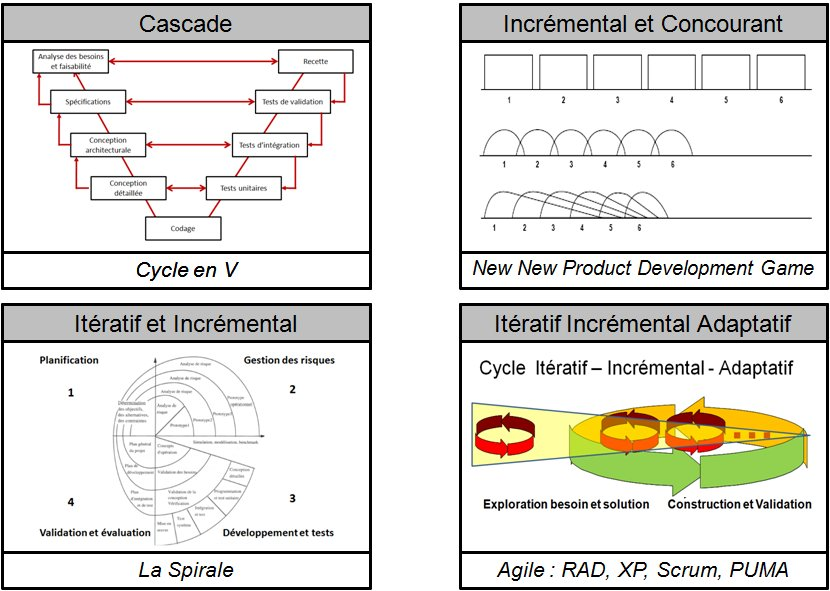
\includegraphics[scale=0.4]{img/cycles-basiques}
    \caption{Les principales cycles de développement logiciel}
	\label{cycles-basiques}
\end{center}
\end{figure}

\subsection{Les grandes familles de cycle de développement}

\subsubsection{Modèle en cascade}

Les phases traditionnelles de développement en cascade sont effectuées simplement les unes après les autres, avec un retour sur les précédentes. Le processus de développement utilisant un cycle en cascade exécute des phases qui produisent des livrables définis au préalable, se terminent à une date précise et seulement lorsque les livrables sont jugés satisfaisants lors d'une étape de validation-vérification.

\begin{figure}[H]
\begin{center}
    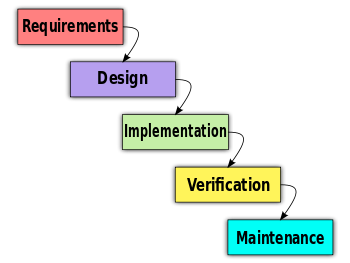
\includegraphics[scale=0.5]{img/waterfall}
    \caption{Le modèle en cascade}
	\label{waterfall}
\end{center}
\end{figure}

\subsubsection{Cycle en spirale}

Par l'implémentation de versions successives, le cycle recommence en proposant un produit de plus en plus complet et dur. En effet, le début de chaque itération comprend une phase d'analyse des risques. Ceci est rendu nécessaire par le fait que, lors d'un développement cyclique, il y a plus de risques de devoir défaire à une telle itération ce qu'on a fait à la précédente.

\begin{figure}[h]
\begin{center}
    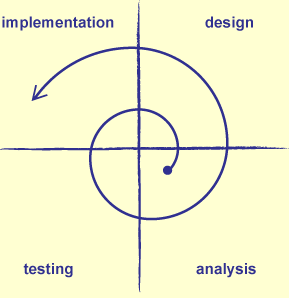
\includegraphics[scale=0.5]{img/spiral-model}
    \caption{Le cycle en spirale}
	\label{spiral-model}
\end{center}
\end{figure}

\subsubsection{Cycle itératif}

Toutes les méthodes Agiles, tels que ASD, FDD, Crystal, Scrum ou \textit{extreme programming},  débutent par des phases séquentielles, courtes mais bien réelles, d'exploration, d'architecture et de planning. Un usage totalement itératif de ces méthodes n'est cependant pas exclu mais ne peut s'appliquer qu'à de très petits projets. En fait, l'idée est de livrer au plus tôt quelque chose qui puisse être testé par le client. On peut en effet réaliser plusieurs itérations sur une documentation telle que l'architecture. 

\begin{figure}[h]
\begin{center}
    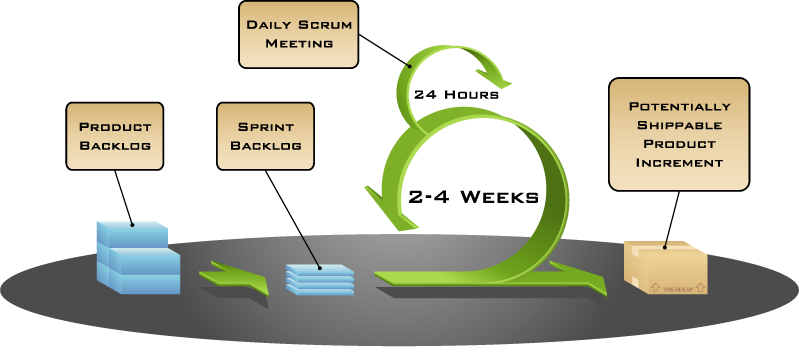
\includegraphics[scale=0.5]{img/scrum}
    \caption{Le processus itératif Agile de type Scrum}
	\label{scrum}
\end{center}
\end{figure}

\subsection{Le cycle de développement à Asert}\label{cycle}

L'entreprise d'accueil ne suit pas l'une des méthodes traditionnelles de processus de développement logiciel. En effet, les directives les plus importantes de toutes les méthodes sont prises en compte lors de la planification du projet, mais la structure globale varie selon le client, la taille et l'équipe.

En général, les étapes initiales des projets commencent très similaires au cycle cascade, avec la spécification des exigences du projet, entre le chef de projet et le client, avec l'aide de l'analyste de systèmes ; la conception des structures du projet, par l'architecte logiciel et l'analyste ; et le codage, par le développeur. Ensuite, le processus devient plus similaire aux méthodes agiles, avec l'intégration de versions préliminaires (alpha, beta, etc.) de la solution et avec des tests hebdomadaires. Finalement, une fois le projet est livré, les routines de maintenance se font périodiquement dans l'année. La documentation de projet n'est pas exhaustive, comme souvent les projets en cascade le demandent, mais un rapport final est livré au cliente avec le logiciel.

Du point de vue d'un projet en cours d'exécution, qui était déjà dans la phase de construction et codage, malheureusement je n'ai pas pu assister à toutes les étapes du cycle de vie du produit. Tout de même, le code du système a été revu plusieurs fois par le client lors de mon séjour à l'entreprise. De petites modifications ont dû être faites, mais cela n'a pas retardé énormément le développement.
%!TEX root = index.tex
\section{Développement}

% intro
% como era o time e do que cada pessoa era responsavel
% passo a passo da minha routine de dev
	% o que os outros faziam, o que eu fazia
% exemplo prático na criacao de alguma tela (das que geram relatorio).

Le deuxième mois de mon stage a été concentré sur le développement du système de gestion d'adhérents de CELGMED (Figure \ref{pp}). J'étais chargé de la conception et création de plusieurs entités Java et fenêtres graphiques Flex, et par la liaison avec les bases de données SQL Server déjà existantes.

\begin{figure}[h]
\begin{center}
    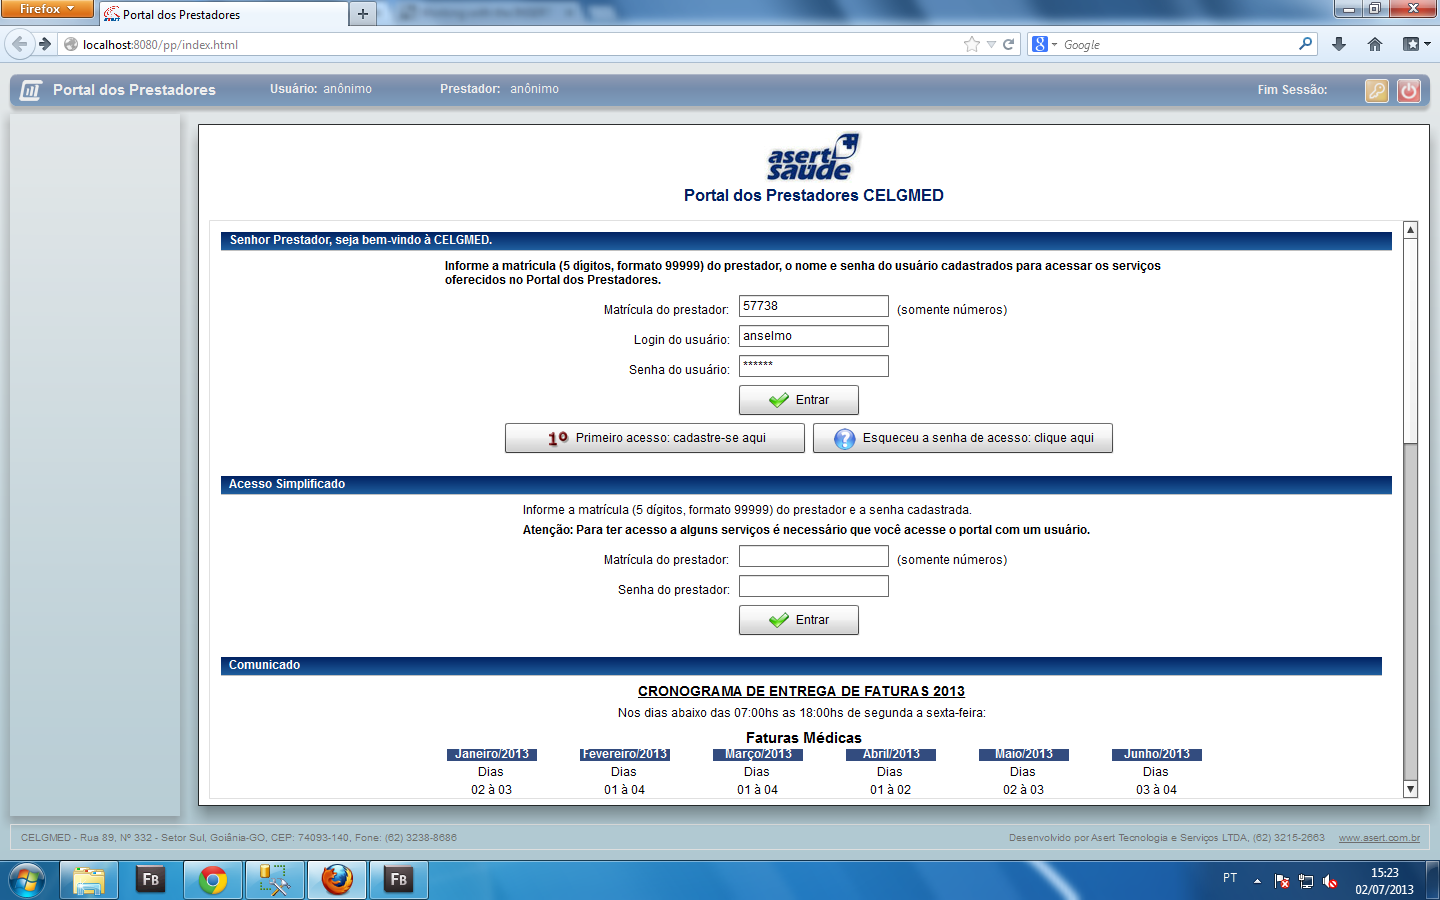
\includegraphics[scale=0.39]{img/pp}
    \caption{Page d'accueil du système d'adhérents CELGMED}
	\label{pp}
\end{center}
\end{figure}

L'équipe informatique était composé du chef de projets, d'un architecte logiciel, d'un développeur base de données, d'une analyste de systèmes, d'un développeur logiciel et de deux stagiaires, moi y compris. Du fait de n'être pas une équipe nombreuse, les tâches étaient souvent confondues et le développement était très agile : l'architecte logiciel touchait aussi au code, le développeur logiciel aidait le responsable des bases de données, et les stagiaires les aidait dans toutes les aires de la programmation.

De manière générale, afin de créer les fenêtres graphiques du système de gestion il fallait suivre quelques phases de développement, soit :

\begin{enumerate}
\item Création de la fenêtre graphique avec l'aide de l'éditeur visuel Adobe Flash Builder. Cette Vue était normalement associée à un ensemble d'entités plutôt qu'à une seule entité. Dans cette phase, il s'agissait d'une fenêtre de prototype, sans actions ou événements.
\item Vérification de quelles tables de la base de données (qui avaient déjà été créées dans la phase de conception) seraient utilisées dans l'application. Voir Section \ref{cycle}, Figure \ref{db}.
\item Création des entités correspondantes aux tables, c'est-à-dire, les classes de Contrôle, Business et Persistance correspondantes. Section \ref{framework}.
\item Codage des interrelations du flux de contrôle décrit dans la Table \ref{flux}. C'était ici que l'on peuplait la Vue avec les actions et événements, ainsi que les classes de \textit{C}, \textit{B} et \textit{P}. Section \ref{section-flux}.
\item Conception du rapport pdf à être généré sur iReport, dans le cas où la fenêtre le demandait, et intégration avec la Vue.
\item Vérification du code par le tuteur.
\end{enumerate}

\begin{figure}[h]
\begin{center}
    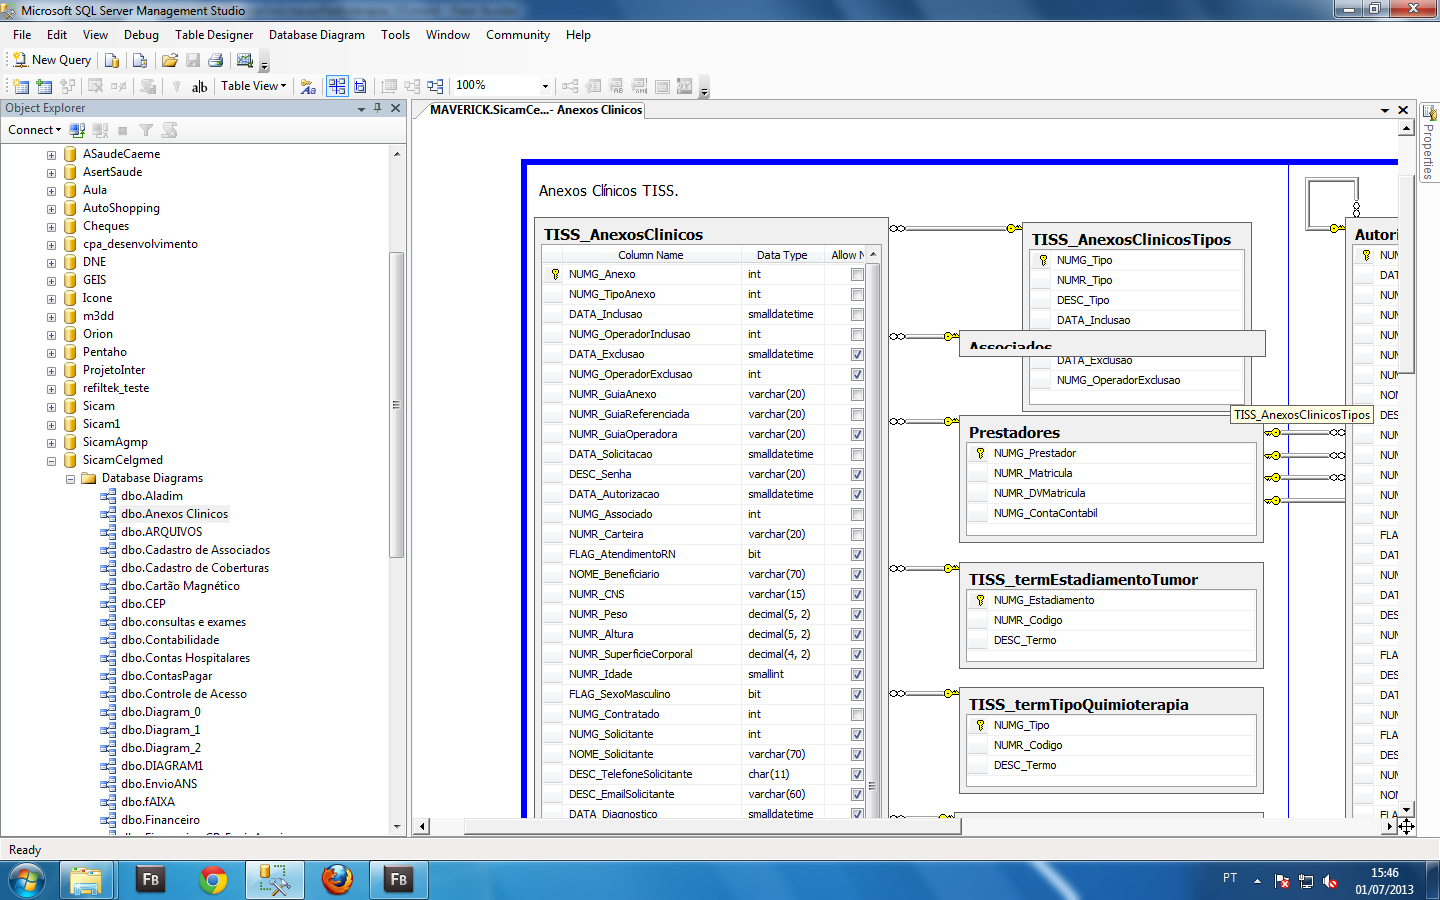
\includegraphics[scale=0.39]{img/db}
    \caption{Base de données relationnelle SQL Server}
	\label{db}
\end{center}
\end{figure}

Encore une fois, ces phases peuvent être mieux expliquées avec un example pratique que j'ai dû exécuter. Supposons la création d'une fenêtre graphique de demande de radiothérapie par un client de la mutuelle de santé CELGMED (Figure \ref{pp-radio}). Ces étapes deviennent donc :

\begin{enumerate}
\item Création de la fenêtre graphique avec l'aide de Flash Builder. Prise en compte des entités qui seraient utilisées : Bénéficiaire (la personne qui a demandé la radiothérapie), Médecin responsable, Maladies diagnostiquées, etc. L'élaboration de cette fenêtre de prototype était très vite, car on prenait souvent une autre fenêtre similaire comme modèle.
\item Vérification des tables à être utilisées : \texttt{celgmed.Beneficiaire}, \texttt{celgmed} \texttt{.Medecin}, \texttt{celgmed.Maladie}, etc.
\item Création des entités correspondantes aux tables : \underline{Ebeneficiaire}, \underline{Emedecin}, \underline{Emaladie}, ainsi que celles correspondantes à la radiothérapie proprement dite, \underline{Cradiotherapie}, \underline{Bradiotherapie}, \underline{Pradiotherapie}. 
\item Codage du flux de contrôle. Un clic dans le bouton « Sauvegarder » faisait que la vue appelle le Cradiotherapie, qui à son tour mettait en place le Bradiotherapie pour vérifier la logique associé à une sauvegarde de données, qui ensuite demandait que la Pradiotherapie fasse les altérations dans les tables avec des commandes SQL : ``\texttt{UPDATE \textit{celgmed.Beneficiaire} SET \textit{VISITE\_MEDICALE}=\textit{1} WHERE \textit{NOM\_BENEFICIAIRE}=`\textit{Pierre \\ Dubois}'}''. Le message d'erreur ou succès retournait à la fenêtre et l'utilisateur voyait le résultat de sa commande : ``Bénéficiaire mis à jour''. Celle-ci était l'étape la plus fastidieuse, car sa sous-division était beaucoup difficile ; la classe P nécessitait de la B, qui nécessitait de la C, qui à son tour était très lié à la V.
\item Conception du rapport PDF à être généré. Il s'agissait de reproduire les mêmes éléments de la fenêtre graphique sous le format JasperReport.
\item Vérification du code par le tuteur.
\end{enumerate}

\begin{figure}[h]
\begin{center}
    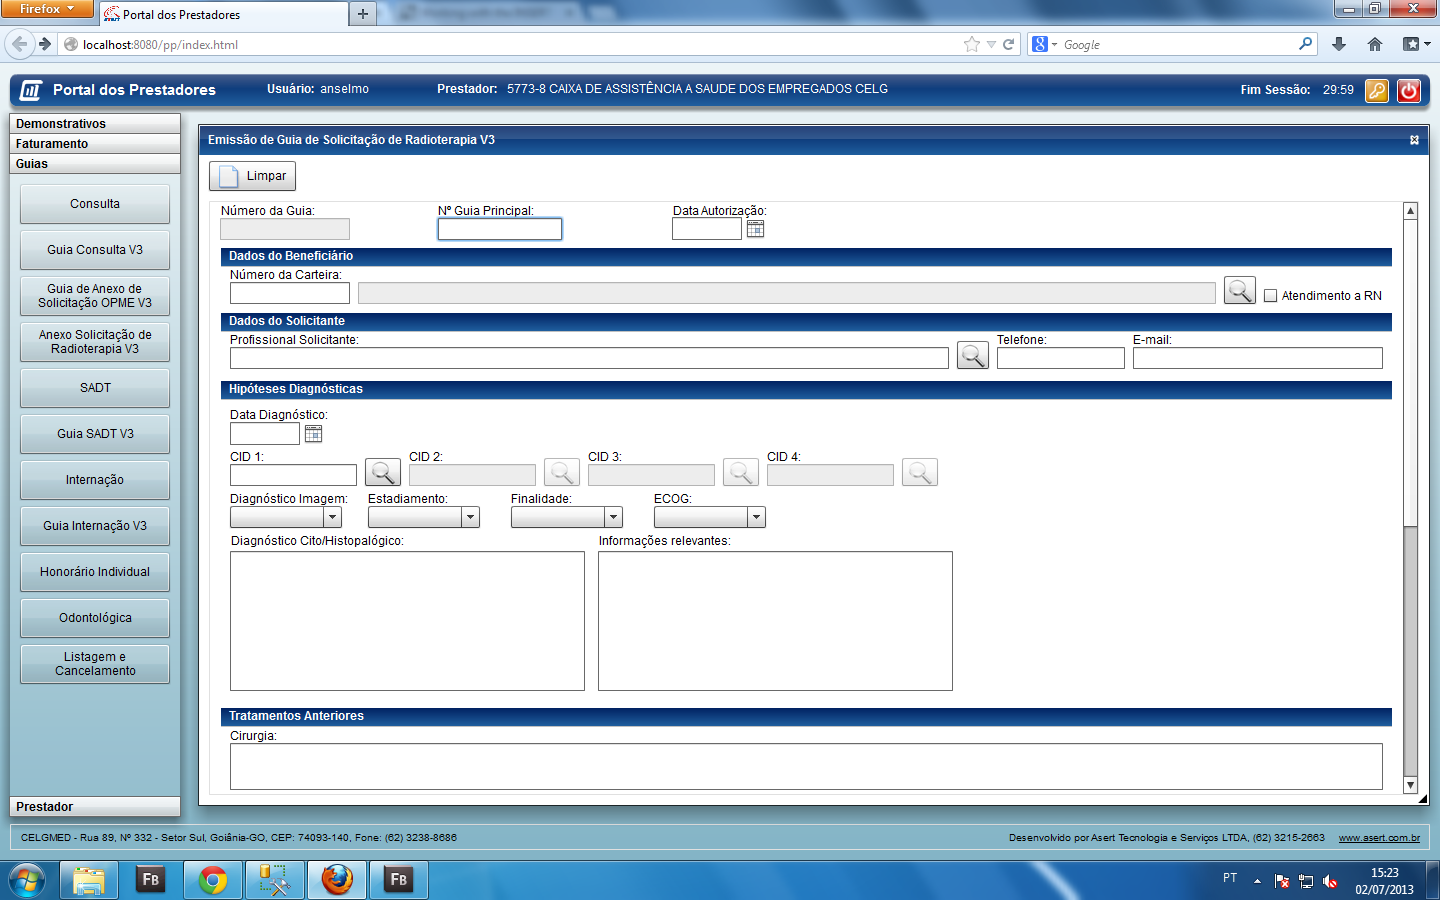
\includegraphics[scale=0.39]{img/pp-radio}
    \caption{Fenêtre de demande de radiothérapie}
	\label{pp-radio}
\end{center}
\end{figure}

Le développement de fenêtres plus élaborées, comme celle de la radiothérapie, prenait environ une semaine pour leur réalisation, alors que les fenêtres plus élémentaires, qui ne touchaient qu'à une seule table de la base de données, comme dans l'enregistrement d'une Rue ou d'une Ville, comptaient une journée. Dans ce rythme, j'ai pu assister à la création de plus d'une dizaine de fenêtres complètes au cours du deuxième mois de mon stage.

\pagebreak
%!TEX root = index.tex
\chapter{Conclusion}

Ce rapport a présente mes expériences professionnelles dans l'établissement Asert Serviços e Tecnologia da Informação, une petite société informatique qui propose des solutions de systèmes de gestion intégrés à d'autres entreprises, principalement à celles d'aide médicale. 

L'opportunité de réaliser un stage ingénieur chez une entreprise de développement logiciel a été très enrichissante, et ces huit semaines de travail ont été très productives. Ce stage m'a donné une grande ouverture d'esprit en voyant une équipe très capacité et m'a motivé dans un cadre académique pour produire des technologies appliquées à des problèmes réels du monde corporatif.

L'environnement amical et stimulant favorise un engagement et un approfondissement interdisciplinaire remarquable. Le fait d'être un petit groupe de développement fait qu'il soit nécessaire de croiser de différentes connaissances et penser aux problèmes à partir d'angles inhabituels. Dans ce sens, le bureau crée une atmosphère qui invite les personnes qui travaillent dans des domaines distincts à interagir et se communiquer même dans des circonstances non-professionnelles. 

Par rapport aux résultats de mon travail, j'ai pu constater une amélioration de ce que je développais, non pas seulement en question de vitesse de travail mais aussi de qualité de code. À la fin de mon séjour, le développeur responsable ne faisait plus de vérifications, car il était à moi de le faire de façon rigoureuse et progressive. 

Le poste que j'ai occupé était sans doute plus proche de celui d'un ingénieur que dans le stage ouvrier à la première année : il y avait des objectifs clairs à remplir, des spécifications, des délais, et des compétences techniques requises. Tout de même, au fur et a mesure que je concevais des fenêtres similaires les unes des autres, j'avais l'impression de ne pas créer de nouvelles fonctionnalités, mais tout simplement de rester sur la méthode de travail ; c'était aux développeurs et à l'architecte d'améliorer le framework de l'entreprise, tandis que j'en étais seulement un utilisateur. J'ai conclu finalement que ce sentiment est normal dans le cadre d'un stage d'apprentissage, vu que j'ai eu très peu de contact avec les bases fondatrices du système, mais cela m'a donne l'envie d'assumer l'un de ces postes dans l'avenir.

La continuation du travail que j'ai effectué a déjà été planifiée et sera finie avant la fin de l'année. L'objectif principal est d'avoir un livrable préliminaire au plus vite possible pour que le client puisse faire des suggestions et l'équipe de développement reformule le système. 

\pagebreak
%!TEX root = index.tex
\printbibliography[heading=bibintoc]


\end{document}
